\section{Adapter Composition and Reuse}
\label{sec:adapter_composition}

\noindent\textbf{SQ2:} \textit{Can independently trained adapters be composed
into multi-task capability without joint retraining or centralised
coordination?} This section surveys composition strategies and where their
assumptions break down for decentralised operation; SQ2 is resolved in the
centralised discussion in Section~\ref{sec:synthesis_gap:answers}.

\subsection{From Single-Task Adapters to Multi-Task Composition}
\label{sec:adapter_composition:intro}

The PEFT methods surveyed in Section~\ref{sec:peft} each produce per-task parameter
sets that are independent of one another and additive with respect to a shared frozen
backbone. This structural property immediately raises a question of \textit{composition}:
given a collection of independently trained adapters, how can their knowledge be combined
to serve a new task or a multi-task query without retraining from scratch? This question
is the central concern of the adapter composition literature, which has grown from simple
sequential stacking to learned attention-based fusion, retrieval-augmented composition,
and the construction of reusable adapter libraries.

Ponti et al.~\cite{Ponti2023} provided a systematic taxonomy of modular deep learning, classifying
composition strategies using three operational families: (i)~\textit{routing} methods, which select
a subset of modules to activate for each input; (ii)~\textit{merging} methods, which
combine module parameters or outputs into a single representation; and
(iii)~\textit{learning-to-combine} methods, which train a meta-module to weight module
contributions. (Ponti et al.\ organise modular architectures across four dimensions of
variation~\cite{Ponti2023}; the three operational families used here: routing, merging,
and fusion are a simplification of that framework.) This taxonomy organises the literature
reviewed in the present section and maps directly onto the design choices available in a
peer-to-peer exchange setting: a receiving peer may route to the most relevant adapter
(Section~\ref{sec:moe_routing}), merge multiple adapters by weight averaging, or apply a
fusion mechanism to combine their outputs layer-by-layer.

\subsection{Centralised Repositories for Adapter Sharing}
\label{sec:adapter_composition:hub}

Pfeiffer et al.~\cite{Pfeiffer2020hub} introduced AdapterHub, a centralised repository and ecosystem for
sharing trained adapter modules across the community. Adapters are uploaded alongside a
unique identifier, base model specification, and task description, and can be retrieved
and inserted into any compatible transformer model at inference time through a
lightweight loading interface. AdapterHub provided the first large-scale demonstration
that adapter modules are practically shareable artefacts: hundreds of community-contributed
adapters (growing to thousands by 2022--2023) were made publicly accessible, enabling practitioners to
reuse community-contributed adapters without any local fine-tuning.

The unified Adapters library of Poth et al.~\cite{PothAdapters2023} extended the AdapterHub
ecosystem to support LoRA, prefix tuning, IA$^3$, and bottleneck adapters under a single
API, with composition primitives for stacking, averaging, concatenation, and gated
combinations. These composition types provide the implementation substrate for the
more complex fusion methods described below.

\subsection{Learned Non-Destructive Composition}
\label{sec:adapter_composition:fusion}

Pfeiffer et al.~\cite{Pfeiffer2021fusion} proposed AdapterFusion, a two-stage approach to multi-task
adapter composition. In the first stage, task-specific adapters are trained independently
in isolation, one per task, each using only that task's data. In the second stage,
a lightweight \textit{fusion layer} (an attention mechanism with learnable parameters) is trained to combine the outputs of all task adapters at each transformer layer:

\begin{equation}
h' = \mathrm{Attention}(h \cdot W_Q,\; [h_1, \ldots, h_K] \cdot W_K,\; [h_1, \ldots, h_K] \cdot W_V)
\label{eq:adapterfusion}
\end{equation}

\begin{figure}[H]
  \centering
  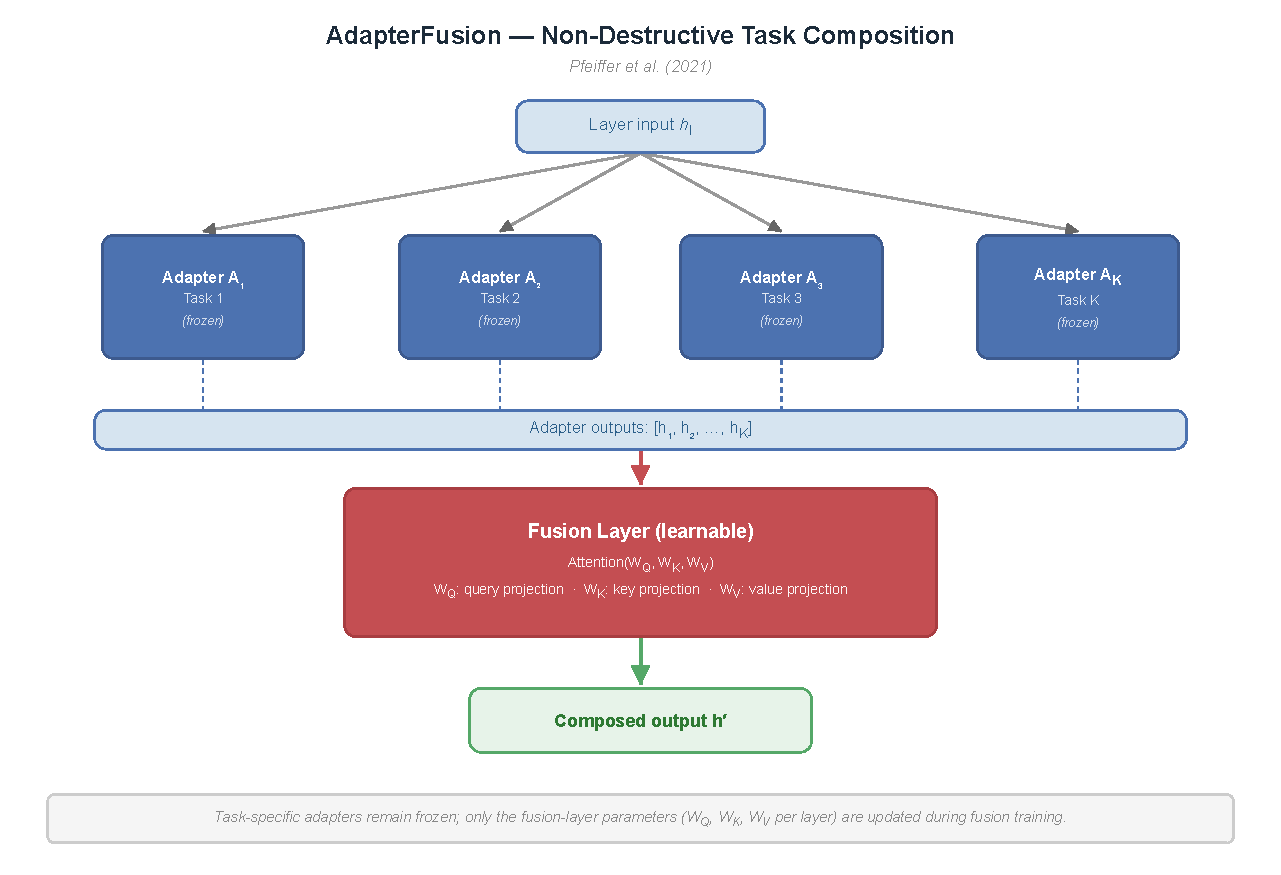
\includegraphics[width=0.85\textwidth]{figures/fig_adapterfusion.pdf}
  \caption{AdapterFusion fusion layer (own figure): task adapters
    $A_1,\ldots,A_K$ remain frozen while a lightweight attention mechanism with
    parameters $W_Q, W_K, W_V$ learns to combine their outputs at each
    transformer layer \cite{Pfeiffer2021fusion}.}
  \label{fig:adapterfusion}
\end{figure}

where $h$ is the current layer representation, $h_k$ is the output of adapter $k$ at
that layer, and $W_Q$, $W_K$, $W_V$ are learnable fusion parameters. The composition
is non-destructive: pre-trained task adapters remain unchanged; only the fusion module
is updated. AdapterFusion adds only the three attention matrices $W_Q$, $W_K$, $W_V$ per layer as fusion parameters, keeping per-task overhead minimal, and achieves multi-task performance
competitive with joint fine-tuning while avoiding catastrophic forgetting, demonstrating
effectiveness across 16 diverse NLU tasks \cite{Pfeiffer2021fusion}.

The non-destructive and modular properties of AdapterFusion make it a key architectural
precedent for the research direction of this review. However, the fusion stage requires
access to all task-specific training sets simultaneously in order to learn the attention
weights, which presupposes a central aggregation step. Removing this centralisation
requirement: learning to combine independently acquired adapters without
shared training data, is one of the open research gaps identified in Section~\ref{sec:synthesis_gap}.

A separate line of work removes AdapterFusion's dependency on centralised training data
entirely by composing adapters algebraically rather than via a trained fusion layer. Task
Arithmetic~\cite{Ilharco2023TaskArithmetic} combines fine-tuned weight deltas through simple
arithmetic operations (addition, negation) without any gradient step or access to the
original per-task training data; TIES-Merging~\cite{Yadav2023TIES} extends this by resolving
sign conflicts between merged parameter updates. These methods demonstrate that multi-task
composition without centralised training data is achievable in principle. They do not,
however, address two properties required by a genuinely decentralised P2P setting: (i)
discovery --- none of these methods locates adapters across a network of autonomous peers,
they assume all adapters to be merged are already locally available; and (ii) independent
initialisation --- reported results typically assume adapters share an initialisation or
fine-tuning lineage (as in model-soup-style averaging, cf. Section~\ref{sec:adapter_composition:library}),
whereas independently trained LoRA modules (with independently sampled low-rank factors)
do not have guaranteed subspace alignment. The centralisation dependency this review
identifies as an open gap is therefore more precisely scoped to fusion of \emph{independently
discovered, independently initialised} adapters without shared training lineage or
centralised coordination, rather than to adapter fusion in general.

\subsection{Cross-Lingual Adapter Stacking}
\label{sec:adapter_composition:madx}

Pfeiffer et al.~\cite{PfeifferMADX2020} introduced the MAD-X (Multilingual Adapter-based Cross-lingual
Transfer) framework, which decouples language-specific and task-specific knowledge into
separate adapter modules. Language adapters are trained on unlabelled corpora for each
target language; task adapters are trained on task-labelled data in a source language.
At inference time, a target-language adapter and a source-language task adapter are
\textit{stacked} sequentially within the same transformer layers, enabling zero-shot
cross-lingual transfer without any target-language labelled data. Ansell et al.~\cite{AnsellMADG2021} introduced MAD-G, which generates language adapters directly
from typological features, enabling zero-shot adapter generation for unseen languages
without any target-language training data, demonstrating that the modular composition principle generalises beyond the bottleneck
adapter architecture.

MAD-X also introduces invertible adapters at the input and output embedding layers,
addressing the token distribution mismatch between source and target languages.
The MAD-X decomposition establishes a broader principle: adapters trained on orthogonal
knowledge axes (language, domain, task) can be stacked and composed without any of the
training processes needing coordination or shared data. Each adapter encodes an independent
slice of competence, and the composite model's behaviour is their sum rather than a
learned joint product.

\subsection{Hypernetwork Approaches to Composition}
\label{sec:adapter_composition:hyper}

Hypernetwork-based methods replace per-task adapter training with a generator network
that produces adapter weights on demand, conditioned on a task or domain embedding.
Zhang et al.~\cite{ZhangHyperPELT2022} demonstrated that a shared hypernetwork generating adapter
weights for all tasks simultaneously reduces total parameter count compared to
independent adapters while preserving per-task performance.
Ivison et al.~\cite{IvisonHyperdecoders2022} applied the same principle to multi-task generation,
showing that a single hypernetwork could generate task-conditioned decoder adapters
across dozens of generation benchmarks.

Hypernetwork approaches introduce a fundamentally different model of composition:
rather than combining pre-existing adapter artefacts, composition is implicit in the
latent space of the hypernetwork. This makes hypernetwork-based adapters less directly
transferable between nodes, since the generator network must accompany the adapter
weights. Unlike self-contained adapter matrices (LoRA, bottleneck), a hypernetwork-generated
adapter cannot be transferred without also transferring the generator network, where the adapter's weight is a function output, not a stored artefact. This makes static
adapter matrices and hypernetwork adapters distinct in their portability, independent
of their accuracy on shared benchmarks.

\subsection{Retrieval-Augmented and Library-Based Composition}
\label{sec:adapter_composition:library}

A complementary line of work frames adapter composition as a retrieval problem. Given a
library of pre-trained adapters, a composition mechanism must select and combine the most
relevant modules for a new query or task.

Huang et al.~\cite{Huang2023} introduced LoraHub, which composes a pool of pre-existing LoRA adapters
through gradient-free, few-shot optimisation: given a handful of examples from a target
task, LoraHub finds a weighted average of adapter matrices whose combination best fits
those examples. This approach requires no gradient updates to any individual adapter and
scales to pools of dozens of adapters, achieving performance comparable to full few-shot
fine-tuning on the Big-Bench Hard (BBH) benchmark \cite{Huang2023}. However, LoraHub
assumes the adapter pool is available locally; it does not address discovering adapters
held by remote peers. Addressing this requires an adapter discovery protocol and a capability representation so that nodes can locate relevant adapters
distributed across the network.

Zhao et al.~\cite{ZhaoLoraRetriever2024} proposed LoraRetriever, which uses input-conditioned
retrieval to select the top-$k$ most relevant LoRA adapters from a library for each
incoming request, then composes them by either averaging adapter outputs (Mixture) or
parameter fusion (Fusion), offering a trade-off between specialisation and integration. The retrieval
step matches input embeddings against adapter descriptions using a shared embedding
space, enabling dynamic routing without task identity signals at query time. A central
limitation for P2P deployment is that LoraRetriever assumes a central retriever with a
pre-indexed catalogue of all accessible adapters. Circumventing this centralisation
requires a decentralised approach to capability representation and
discovery, so that queries can be routed without a search engine.

Ostapenko et al.~\cite{Ostapenko2024} studied how to build and reuse a structured library of LoRA
adapters, introducing model-based clustering (MBC) to group tasks by adapter parameter
similarity and a zero-shot routing mechanism (Arrow) for dynamic adapter selection at
test time. The resulting library functions as a persistent knowledge store that
grows with accumulated experience conceptually analogous to the adapter registry
component of a P2P exchange architecture.

Wortsman et al.~\cite{Wortsman2022} demonstrated that averaging the weights of multiple fine-tuned
models (``model soups'') improves robustness and out-of-distribution generalisation
without any additional training. (While Model Soups was demonstrated for vision models,
the weight-averaging principle extends by construction to any linear parameter space,
including LoRA adapter matrices, provided the adapters share the same initialisation
point.) Applied to adapter-scale modules, this result implies
that adapter weight averaging is a viable zero-shot composition strategy: a peer can
combine adapters from different sources by mean-averaging their weight matrices,
without requiring access to any of the original training data.

\subsection{Unified Multi-PEFT Composition}
\label{sec:adapter_composition:unified}

Mao et al.~\cite{MaoUniPELT2022} proposed UniPELT, a unified framework that activates and
composes multiple heterogeneous PEFT methods (bottleneck adapters, prefix tuning, LoRA)
within a single model using per-layer gating scalars. The gating mechanism learns to
assign each PEFT type an activation weight per layer and per task, effectively selecting
the most appropriate combination for each setting. UniPELT matches or outperforms any
single PEFT method across several GLUE benchmarks\footnotemark, demonstrating that composition of
heterogeneous PEFT types can exceed the performance of any single homogeneous method
\cite{MaoUniPELT2022}.
\footnotetext{UniPELT reports improvements on a subset of GLUE tasks rather than
uniform superiority across all eight; its benefit is a consistent advantage
across settings, not a universal winning margin \cite{MaoUniPELT2022}.}

\noindent The composition findings of this chapter are consolidated, alongside
the other four sub-questions, in the centralised discussion in
Section~\ref{sec:synthesis_gap:answers}.

